\chapter{C-AD Guidance}
\label{chap:cad}

For planning purposes in this document, we use luminosity projection numbers provided by the Collider-Accelerator Division (C-AD).   The version of the document titled 
"RHIC Collider Projections (FY 2017 –- FY 2027)" utilized for this study is dated XX August 2020 and utilizes knowledge gained from the Run-15 \pp and \pau at 200 GeV running and the Run-16 \auau at 200 GeV running.   The document is available at:

\bigskip
{\color{blue}{http://www.rhichome.bnl.gov/RHIC/Runs/RhicProjections.pdf}} 
\bigskip

Note that the document linked above is periodically updated, so note the date tag.  In general, C-AD provides a minimum and maximum luminosity per week for each running period, as well as the fraction of collisions within a given z-vertex range. For calculating the integrated luminosity, we assume a ramp-up curve and then a steady-state physics running at the mean of the minimum and maximum in both luminosity and z-vertex fraction $f_{z}$ (where a minimum and maximum are given).   

As placeholders, here are two figures JH received from C-AD.

\begin{figure}
    \centering
    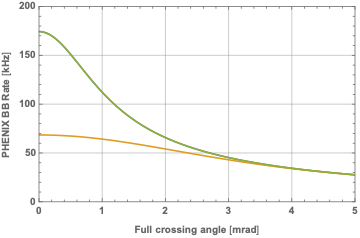
\includegraphics[width=0.8\linewidth]{figs/figure_cad1_prelim.png}
    \caption{Caption}
    \label{fig:cad1}
\end{figure}

\begin{figure}
    \centering
    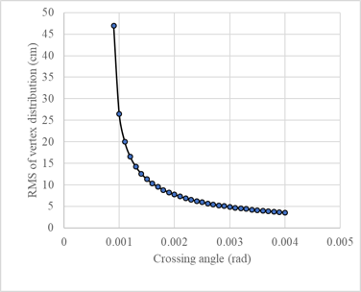
\includegraphics[width=0.8\linewidth]{figs/figure_cad2_prelim.png}
    \caption{Caption}
    \label{fig:cad2}
\end{figure}